\documentclass[UTF8]{ctexart}
\usepackage{geometry}
\usepackage{fancyhdr}
\usepackage{verbatim}
\usepackage{enumerate}
\usepackage{graphicx}
\usepackage{subfigure}
\usepackage[colorlinks,linkcolor=blue]{hyperref}
\usepackage{listings}
\usepackage{fontspec}
\setmonofont{Consolas}
\usepackage{color}
\usepackage{xcolor}
\graphicspath{{./Images/}}

\geometry{papersize={210mm,297mm}}
\geometry{left=2.5cm,right=2.5cm,top=2.5cm,bottom=2.5cm}

\setlength{\headheight}{13pt}

\title{SlopeCraft v3.6教程}
\author{TokiNoBug}
\date{\today}

\begin{comment}
\pagestyle{fancy}

\lhead{\author}
\chead{\title}
\rhead{\date}

\lfoot{}
\cfoot{\thepage}
\rfoot{}

\renewcommand{\headrulewidth}{0.4pt}
\renewcommand{\headwidth}{\textwidth}
\renewcommand{\footrulewidth}{0pt}

\end{comment}

\begin{document}
    \maketitle
    %%%%%%%%%%%%%%%%%%%%%%%
    % Page1
    %%%%%%%%%%%%%%%%%%%%%%%
    SlopeCraft v3.6是一个重大更新,整个程序都被重构了一遍,增加了许多硬核的功能,解决了不少棘手的麻烦:v3.6实现了期盼已久的有损压缩功能,可以把地图画总高度压缩到几乎任何值,彻底解决了地图画超出限高的问题;v3.6加入了“搭桥”功能,可以辅助玩家建造……
    
    除此以外,v3.6还修改了界面的操作逻辑。加之上一版教程还是v3.1,我认为有必要写个新的教程。

    这篇教程不是“傻瓜式”的,我只介绍必须介绍的,强调必须强调的。

    %%%%%%%%%%%%%%%%%%%%%%%
    % Page2
    %%%%%%%%%%%%%%%%%%%%%%%
    \pagebreak
    \section{v3.6更新内容简介}
    \paragraph{新内容}
    \textbf{SlopeCraftL3.dll}——SlopeCraft的内核开发成了通过接口类调用的\textbf{动态链接库},包含了立体、平板、纯文件地图画和墙面像素画的核心功能,理论上应该能被C++、Java、Python等语言调用(C++亲测可用,其他语言顶多再套一层接口),以后的插件可以\textbf{少造轮子}了!

    \paragraph{新功能}
    \begin{enumerate}
        \item 第61个基色:\textbf{发光地衣}——补上了v3.5.1的遗漏
        \item 智能有损压缩——\textbf{彻底解决超限高问题}
        \item 搭桥——\textbf{方便建造立体地图画}
        \item 防火/防末影人——用玻璃块包围\textbf{易燃方块}和\textbf{可被小黑偷走}的方块
        \item 导出为.NBT格式——\textbf{Litematica}和\textbf{原版结构方块}可以用,不知WorldEdit是否可用
        \item 方块增加了各种\textbf{下半砖}
        \item 自定义方块列表——更加自由,想要什么方块\textbf{自己加}
        \item 构建三维结构时预览地图画——\textbf{有损压缩可能会微调画面内容}
        \item 检查更新、反馈Bug——请认准\href{https://github.com/ToKiNoBug/SlopeCraft}{GitHub仓库}
        \item 更加完善的报错系统——\textbf{报错信息不是天书!}
        \item 启动时自动设置语言——默认简体中文,如果系统语言没有汉语,那就英文
        \item settings.json——启动时的配置文件
        \item 新的像素画类型:墙面像素画——其实有点不伦不类,偏偏很多人想要这个功能
    \end{enumerate}
    \paragraph{修复Bug}
    \begin{enumerate}
        \item 修复了无法禁用部分颜色的Bug——重写了方块列表的逻辑 
    \end{enumerate}
    \paragraph{优化和其他更改}
    \begin{enumerate}        
        \item 优化了转化图片和搭桥的性能
        \item 删除了可去掉的“确认”按钮,节省操作
        \item 等待用户操作时进度条不再显示为繁忙状态,更符合操作习惯
    \end{enumerate}

    \pagebreak
    %%%%%%%%%%%%%%%%%%%%%%%
    % Page3
    %%%%%%%%%%%%%%%%%%%%%%%
    \section{初级教程}
    \subsection{导入图片}
    从上一个教程(v3.1)到v3.6,最大的变化其实还是多了个“设置”按钮,用来更好的处理原图中\textbf{透明像素}。
 
    点击\textbf{设置}按钮,可以看到子窗口,如图\ref*{SetTPS}:

    \begin{figure}[htbp]
        \centering
        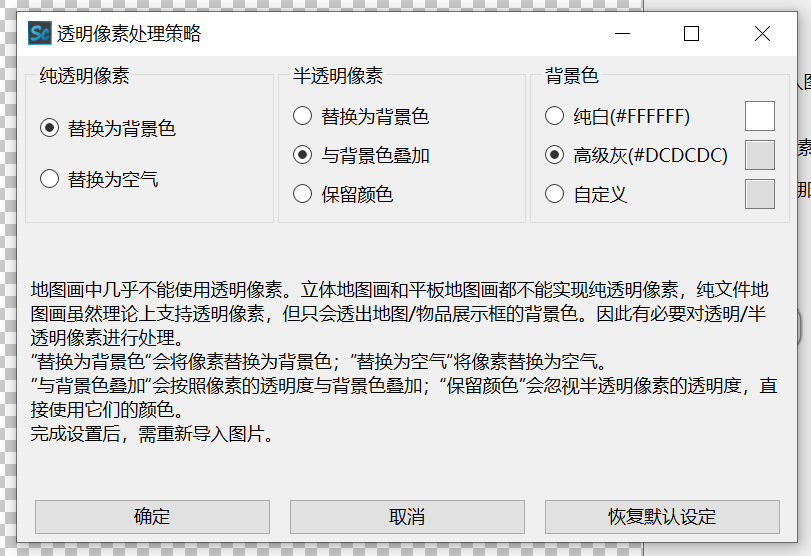
\includegraphics[width=15cm]{Img1_TPS.png}
        \caption{设置透明像素处理策略的界面}
        \label{SetTPS}
    \end{figure}
    
    \textbf{请注意:如果你要按照自定义的策略导入含全透明/半透明像素的图片,务必先设置透明像素处理策略,后导入图片!否则图片只会按照默认的处理策略处理!如果已经导入了图片才重新设置处理策略,请重新导入图片。}

    透明像素处理策略有不同的方法处理纯透明像素(alpha=0)和半透明像素(alpha>0)。纯透明像素要么替换为背景色,要么设为空气;半透明像素既可以替换为背景色,也可以与背景色叠加融合,还可以忽略掉它的透明度属性,直接当做不透明像素。另外也可以设置背景色,默认背景色是雪块平铺时的浅灰色,也可以选择纯白色,或者任何自定义颜色。

    强调一下,原图中\textbf{每个像素对应着地图画的一个方块},导入图片之前需要自己裁剪、缩放图像,图片的长和宽最好是\textbf{128像素的整数倍}(不是强制要求)。这一步预处理应当由用户自己完成,我不在软件中实现这个功能,也不存在任何缩放图像的操作,SlopeCraft忠实的映射\textbf{每个像素}。

    \subsection{设置地图画类型}
    地图画类型中多了一项墙面像素画,除此以外没有改动。只需要按说明设置地图画类型及版本,然后直接跳转到下一页即可。

    设置方块列表页面补加了第61个基色:发光苔藓。这是1.17已经添加的基色,但v3.5.1漏了。
    请注意方块列表的逻辑:灰色的按钮/选择框代表锁定、不可更改的,如基色0(透明)必须启用。SlopeCraft要求每种基色必须有对应的方块,哪怕这种基色本身被禁用。因此如果某个基色只有一种方块可选,那个唯一的单选框也是锁定的。
    
    如果一种方块版本过高,它同样会变为灰色,不可选择。有必要指出,有些方块是墙面像素画不能使用的,如铁质压力板、发光苔藓等。这时限制颜色数量的不仅有基色/地图色本身的性质,还有你所选的方块。

    \subsection{调整颜色}
    调整颜色界面也没有值得一提的改变,和旧版本一样操作就好。
    
    首先选择好转化算法,然后选择是否启用抖动,点击\textbf{转化},等待转化完成,就可以选择你想要的导出方式。
    
    六个转化分别对应着六种不同的色差公式。算法中RGB+最为推荐,RGB和XYZ速度最快,Lab94和Lab00效果较好但性能较慢,HSV效果一直不太理想,不太推荐。
    
    抖动则使用Floyd-Steinberg算法,尝试用几种相近的颜色掺混,试图更好的贴合原图。
    
    这里以\href{https://t.bilibili.com/544583492149793294}{Lancet\_Corgi画的图}为例。(\href{https://space.bilibili.com/37171000}{Lancet\_Corgi的b站主页},感谢\~)
    
    \begin{figure}[htbp]
        %\addtocounter{figure}{-1}
        \centering
        \setcounter{subfigure}{0}
        \subfigure[原图]{
            \begin{minipage}[t]{7cm}
                \centering
                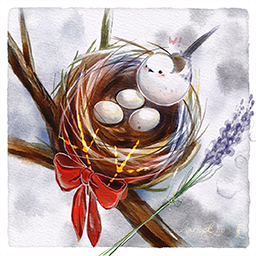
\includegraphics[width=6cm]{Img3_Raw.png}
                %\caption{原图}
                
                \label{ruby_raw}
            \end{minipage}
        }
        \subfigure[转化后]{
            \begin{minipage}[t]{7cm}
                \centering
                
\includegraphics[width=6cm]{Img4_Converted.png}
                %\caption{转化后}
                \label{ruby_converted}
            \end{minipage}
        }
        \caption{导入原图并按RGB+算法(无抖动)转化}
    \end{figure}
    
    \subsection{导出三维结构}
    若想要把地图画保存为\textbf{.Litematic}(投影mod)、\textbf{.nbt}(结构方块)格式,须先点击\textbf{构建三维结构},然后再\textbf{导出}。构建三维结构完成之后会自动弹出预览窗口,可以查看材料表,也可以查看地图画。

    \begin{figure}[htbp]
        \centering
        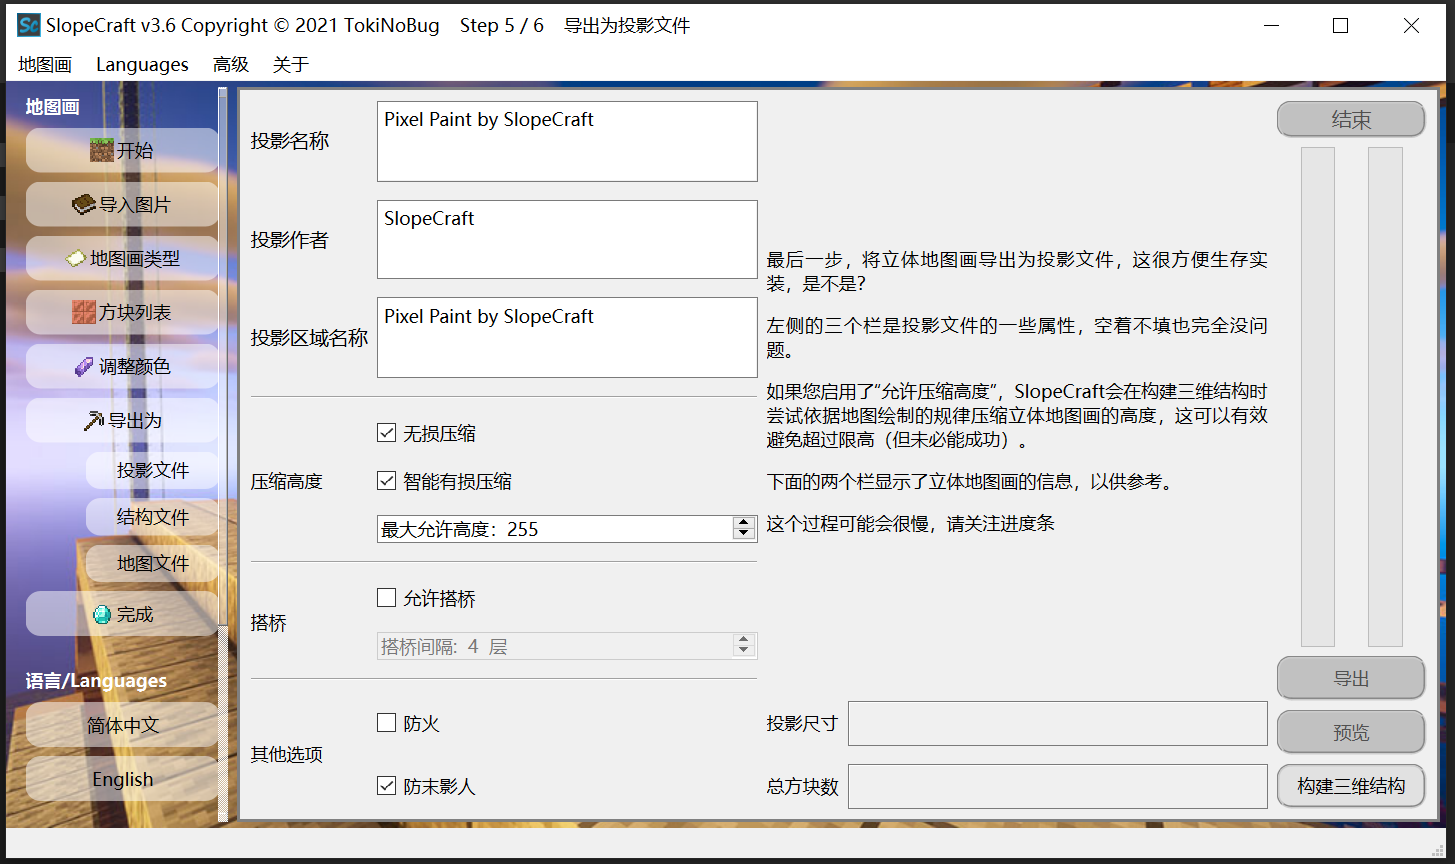
\includegraphics[width=15cm]{Img2_Export3D.png}
        \caption{导出三维结构界面}
    \end{figure}

    压缩高度一栏增加了\textbf{智能有损压缩};增加了\textbf{搭桥}选项;增加了\textbf{防火}和\textbf{防末影人}选项。 在主进度条的右侧多了一个子进度条,表示有损压缩/搭桥的进度。
        
    \subsubsection{压缩}
    简单来说,无损压缩是在\textbf{严格保证每个像素颜色不变}的前提下,以连续性为代价,压缩地图画总高度,但它约束较大,未必如愿。毫不夸张的说,有些图片是不可压缩的,比如纯白色的部分。这时候就需要新的压缩技术:智能有损压缩。

    有损压缩则\textbf{微调个别像素的颜色},压缩地图画总高度,使其小于等于用户指定的最大允许高度。有损压缩使用遗传算法实现,属于群体人工智能,是目前SlopeCraft中技术含量最高的模块。最大允许高度不要低于14,否则立体地图画很可能压缩失败。

    一般来说,有损压缩的最大允许高度越小,画质损失越明显。如下,这张图若做成立体地图画,高度是255格,现在进行有损压缩(同时启用无损压缩)。图\ref*{ruby_max100}为最大高度100格时的构建结果,图\ref*{ruby_max20}为最大高度20格时的构建结果。

    \begin{figure}[htbp]
        \centering
        \subfigure[最大100格]{
            \begin{minipage}[t]{7cm}            
                \centering
                
\includegraphics[width=6cm]{Img6_Compressed_100.png}
                \label{ruby_max100}
            \end{minipage}
        }
        \subfigure[最大20格]{
            \begin{minipage}[t]{7cm}
                \centering
                
\includegraphics[width=6cm]{Img5_Compressed_20.png}
                \label{ruby_max20}
            \end{minipage}
        }
        \caption{最大允许高度对画质的影响}
    \end{figure}

    压缩前后图片没有显著变化,画质损伤不明显。但仔细观测仍可以发现,左右两侧留白部分出现了一些灰点,且图\ref*{ruby_max20}由于压缩程度高,灰点较图\ref*{ruby_max100}更多。另外,遗传算法是一种随机优化算法,被修改像素有一定随机性,不会呈现明显的规律图样。

    有损压缩和无损压缩可以搭配使用,也可以分别独立使用。但一般来说,如果启用了有损压缩,没道理不启用无损压缩。纯有损压缩需要修改更多的像素,对画质的损伤会比较大,无损压缩能在修改像素更少的情况下完成压缩任务,很大程度上减轻画质损伤。
    
    平板地图画和墙面像素画可以勾选这两个选项,但\textbf{不会发挥任何作用}。

    \subsubsection{搭桥}
    立体地图画的每个水平截面上都有很多分散的方块,极不方便建造,倘若能用多条通路连接这些分散的方块,无疑能让建造更加容易。搭桥就是在一个水平面内用玻璃方块连接所有方块,形成通路从而辅助玩家建造的过程。
    
    毫无疑问,搭桥会消耗额外的玻璃,因此不推荐在立体地图画的每一层都执行搭桥。默认每间隔4层搭一次桥,你也可以修改这个间隔。间隔过大,辅助搭桥的效果会减弱;间隔过小,浪费玻璃。
    
    有关地图画压缩和搭桥的详细信息,可阅读\href{https://github.com/ToKiNoBug/SlopeCraftTutorial/blob/main/BasicPrinciple/Principle%20of%20map%20pixel%20arts.md}{地图画原理}。

    \href{https://github.com/AbrasiveBoar902}{AbrasiveBoar902}为优化搭桥性能提供了极大帮助,感谢AbrasiveBoar902的帮助。

    \subsubsection{防火/防末影人}
    顾名思义,这是在保护可燃方块,并避免小黑偷东西。具体方法是用玻璃包裹这些方块的每一个暴露在外的表面,亲测有效。不过这也同时会耗费大量的玻璃,需要谨慎选择。

    \subsubsection{导出}
    目前支持的有\textbf{*.Litematic}(投影mod)和\textbf{*.nbt}(原版结构方块)两种格式。

    \begin{figure}[htbp]
        \centering
        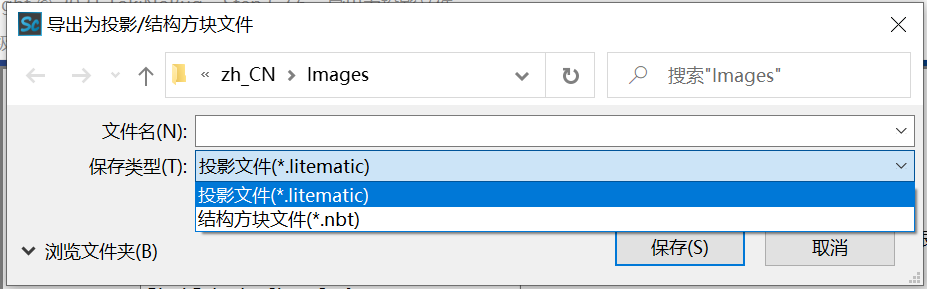
\includegraphics[width=15cm]{Img7_SelectFormat.png}
        \caption{设置导出格式}
        \label{setExport3DFormat}
    \end{figure}

    若要保存为结构方块格式,须在导出时选择相应的文件后缀名,如图\ref*{setExport3DFormat}所示。

    \subsection{导出纯文件地图画}
    和以前的版本相比,导出为纯文件并没有什么变化。

    地图文件的文件名形如map\_i.dat,其中i是大于等于0的整数,如map\_3.dat。\textbf{i就是这个地图文件的序号。序号实际上是地图文件的唯一标识符}。正常情况下,我们生成的地图文件不应该覆盖掉无关的地图文件,所以设置初始序号需多加注意。

   在游戏中按下F3+H可以查看物品的详细信息,\textbf{包括地图物品的Id,也就是对应的地图文件的序号}。图\ref*{mapItem}中显示的地图物品对应名为map\_6.dat的地图文件。
   \begin{figure}[htbp]
       \centering
       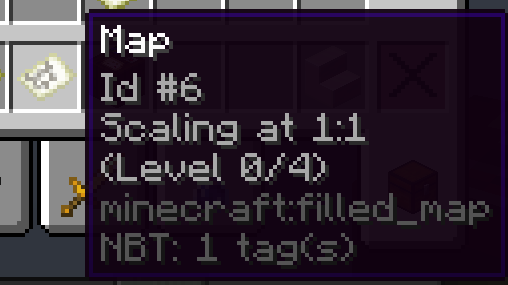
\includegraphics[height=4cm]{Img8_MapItem.png}
       \caption{地图物品与地图序号}
       \label{mapItem}
   \end{figure}

   \begin{itemize}
       \item 如果你想通过/give命令来获得地图:
       
       起始序号可以随意设置,只要不覆盖掉无关的地图。
       \begin{enumerate}
           \item 在1.12,使用 /give @s filled\_map 1 i 来获得序号为i的地图。
           \item 在1.13+,使用 /give @s filled\_map\{map:i\} 来获得序号为i的地图。
       \end{enumerate}
       \item 如果你不想使用命令,只替换地图文件:
       \begin{enumerate}
           \item 先创建与地图画对应的n个地图,n就是SlopeCraft显示的地图文件数量,在本例中是4。
           \item 在游戏中按下F3+H,查看地图文件对应的序号。这些地图对应的序号应当是 a\textasciitilde(a+n-1) ,共n个。
           \item 关闭游戏,在SlopeCraft的\textbf{地图文件起始序号栏}中填入a的值。
           \item 点击导出,选中存档下的data文件夹。SlopeCraft将会替换掉这n个地图文件。
           \item 关闭SlopeCraft,打开游戏,这n个地图应当已经被成功的替换为地图画。
           \item 如果你担心输错地图文件序号,导致无关的地图被覆盖掉,你可以先新建一个临时的文件夹,在导出时选择这个临时文件夹。确认地图序号无误后,再复制黏贴替换掉你要替换的地图文件。
       \end{enumerate}
   \end{itemize}
   
   \pagebreak
   \section{高级功能}
   如果你只是简单的使用SlopeCraft,掌握初级功能足矣;但如果你需要自定义一些东西,那么你最好阅读下这一节。使用高级功能往往需要理解地图画的基本原理,我强烈建议你先看完\href{https://github.com/ToKiNoBug/SlopeCraftTutorial/blob/main/BasicPrinciple/Principle%20of%20map%20pixel%20arts.md}{地图画原理}。

   \subsection{自定义方块列表}
   如果你不满足于我预设的那些方块,想要自己添加其他的原版方块甚至mod方块,这一章会告诉你怎么在SlopeCraft中添加并使用自定义的方块。
   
   \subsubsection{前置信息}
   你需要掌握方块的以下信息:

   \begin{enumerate}
       \item 方块的\textbf{完整}id,包含\textbf{命名空间前缀}以及\textbf{所有方块属性}。
       
       如涂蜡铜块上半砖:
       
       minecraft:waxed\_copper\_slab[type=top,waterlogged=false]

       这里面minecraft:是原版方块的命名空间前缀,中括号里的内容是所有方块属性。保险起见,你应当给每个方块属性都设置对应的值。
       \item 方块最早出现的游戏版本。
       
       SlopeCraft在方块列表中约定了以下几个值代指大版本:
       \begin{table}[h]
        \centering
        \caption{数字与版本的关系}
        \label{VerAndRealVer}
        \begin{tabular}{cc}\hline
            数字 & 版本 \\ \hline
            0 & 早于1.12 \\
            12 & 1.12 \\
            13 & 1.13 \\
            14 & 1.14 \\
            15 & 1.15 \\
            16 & 1.16 \\
            17 & 1.17 \\
            255 & 未来版本 \\
            \hline            
        \end{tabular}
       \end{table}

   正常情况下,你不应该使用255,它只是一个预留的值。如果你非要给一个方块指定为未来版本,那么导致的一切都属于未定义特性——我也不知道会发生什么。

   \item 方块在1.12的id
   
   添加这个属性是因为Mojang从1.12更新到1.13修改了相当多方块的id。如果你要添加的方块在1.12未添加,或者id没有改变,可以填空字符串。
   \item 方块的基色
   
   这可能是最容易出错的地方。对于原版方块,你可以查询\href{https://wiki.biligame.com/mc/%E5%9C%B0%E5%9B%BE%E7%89%A9%E5%93%81%E6%A0%BC%E5%BC%8F#idcounts.dat_.E6.A0.BC.E5.BC.8F}{Minecraft Wiki}。如果是mod自定义的方块,要么自己想办法测,要么去问mod开发者。
   
   如果不懂什么是基色,去看\href{https://github.com/ToKiNoBug/SlopeCraftTutorial/blob/main/BasicPrinciple/Principle%20of%20map%20pixel%20arts.md}{地图画原理}。
   \item 方块中文名称
   \item 方块英文名称
   \item 方块的下方需要依附其他方块
   \item 方块是否发光
   \item 方块是否可燃
   \item 方块是否可被末影人偷走
   \item 方块是否可用于墙面像素画(如水、铁质压力板等方块是不适合的)
   \item 方块的材质图片(建议为一张16*16像素的png图片)   
   \end{enumerate}

   \subsubsection{方块与方块列表}
   SlopeCraft中,方块列表以json格式存储,相关的图片放在FixedBlocks和CustomBlocks文件夹下。
   
   方块列表分为两类:固定方块列表与自定义方块列表。其中固定方块列表是我提供的最基础的一些方块,存储与\textbf{FixedBlocks.json}中(对应的图片在\textbf{FixedBlocks}文件夹下),确保每个基色都存在对应的方块。虽然方块列表中的方块事实上是在程序运行时才确定,但\textbf{你不应该修改它}。
   
   自定义方块列表存储在\textbf{CustomBlocks.json}中,相应的图片在\textbf{CustomBlocks}文件夹下,这是用户自定义的方块列表,允许用户灵活编辑。我在里面写了一些半砖方块,可以作为参考。
   
   每个方块拥有以下属性:
   \begin{table}[h]
    \centering
    \caption{方块的属性}
    \begin{tabular}{ccccc}
        \hline
        属性名 & 类型 & 是否必填 & 默认值 & 说明  \\ \hline
        baseColor & byte & 是 & & 方块的地图基色 \\
        id & string & 是 & & 方块id,包括命名空间和详细方块状态\\
        version & byte & 是 & & 方块最早出现的版本。 \\
        nameZH & string & 是 & & 方块的中文名 \\
        nameEN & string & 是 & & 方块的英文名 \\
        icon & string & 是 & & 方块对应图片的文件名 \\
        idOld & string & 否 & 空字符串 & 方块在1.12的id \\
        needGlass & bool & 否 & false & 指示方块底部是否必须有其他方块 \\
        isGlowing & bool & 否 & false & 指示方块是否发光 \\
        endermanPickable & bool & 否 & false & 指示方块是否可以被末影人偷走 \\
        burnable & bool & 否 & false & 指示方块是否可以被烧毁 \\
        wallUseable & bool & 否 & true & 指示方块是否可以用于墙面像素画 \\
        \hline 
    \end{tabular}       
   \end{table}
   
   \clearpage
   用json格式表示如下:
\begin{lstlisting}[language = C++, numbers=left, 
    numberstyle=\tiny,keywordstyle=\color{blue!70},
    commentstyle=\color{red!50!green!50!blue!50},frame=shadowbox,
    rulesepcolor=\color{red!20!green!20!blue!20},basicstyle=\ttfamily]
{
    "baseColor":11,
    "id":"minecraft:cobblestone_slab[type=top,waterlogged=false]",
    "nameZH":"圆石上半砖",
    "nameEN":"Cobblestone slab",
    "icon":"cobblestone.png",
    "version":0,
    "idOld":"minecraft:stone_slab[half=top,variant=cobblestone]"
}
    \end{lstlisting}
    上面这段json信息展示了一个圆石上半砖的方块信息,解析如下:

    \begin{enumerate}
        \item 它的基色是11,这也是圆石、石砖、石头的基色。
    
        \item 它的方块id是“minecraft:cobblestone\_slab[type=top,waterlogged=false]”,中括号里的方块状态指出这是个上半砖,且不含水;
    
        \item 它的中文名是“圆石上半砖”,英文名是“Cobblestone slab”;
    
        \item 它的图片是一个名为“cobblestone.png”的图片,这个图片放在CustomBlocks文件夹下;
    
        \item 它最早出现的版本为0,代表它在1.12之前就已经加入;
    
        \item 由于它的方块id在1.13发生了变化,它在1.12的方块id为idOld的值。

\end{enumerate}

    这段json中并没有显式列出方块的所有信息,其中needGlass、isGlowing、endermanPickable、burnable、wallUseable这些信息都使用了默认值,分别说明这个方块不需要依附其他方块、不发光、末影人偷不走、不可燃、可用于墙面像素画。

    \subsubsection{自己动手,丰衣足食}
    掌握以上信息后,就可以向自定义方块列表里写入任何你想要的方块了。步骤如下:

    \begin{enumerate}
        \item 将方块的图片做成16*16像素的png图片,放入CustomBlocks文件夹内。
        \item 将方块的json信息填入CustomBlocks.json中,注意json格式不要出错。
        \item 重启SlopeCraft,如果一切正常,你的方块将会成功加入到方块列表里;否则注意察看报错信息。
        \item 重复制作地图画的流程。
    \end{enumerate}

    \subsection{测试方块列表}
    投影中方块缺失基本上都是\textbf{id拼写错误}造成的。如果你一次性导入很多方块,这个功能可以快速测试出方块列表中每个方块有没有id错误。

    测试方块列表会生成一个特殊的结构方块文件,包含每种基色拥有的每一种可用方块(因版本不符合的除外)。结构文件中每个方块均按方块列表中的顺序排列。
    
    如果一切正常,不会有任何一个方块缺失;反之则说明对应的方块存在id错误。
    
    \begin{figure}[htbp]
        \centering
        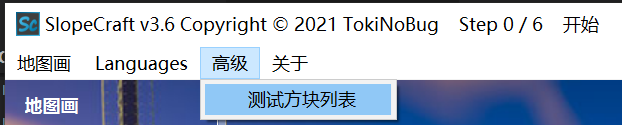
\includegraphics[width=15cm]{Img9_TestBlockList.png}
        \caption{测试方块列表在高级菜单下}
        \label{locOfTestBlockList}
    \end{figure}

    设置好游戏版本后,点击菜单栏\textbf{高级}下的\textbf{测试方块列表},选择保存这个结构方块文件的位置,如图\ref*{locOfTestBlockList}。SlopeCraft就会生成一个这样的结构方块文件。导入到游戏中即可,效果如图\ref*{testBlockListNBT}。

    \begin{figure}[htbp]
        \centering
        \subfigure[左半段]{
            \begin{minipage}[t]{7cm}
                \centering
                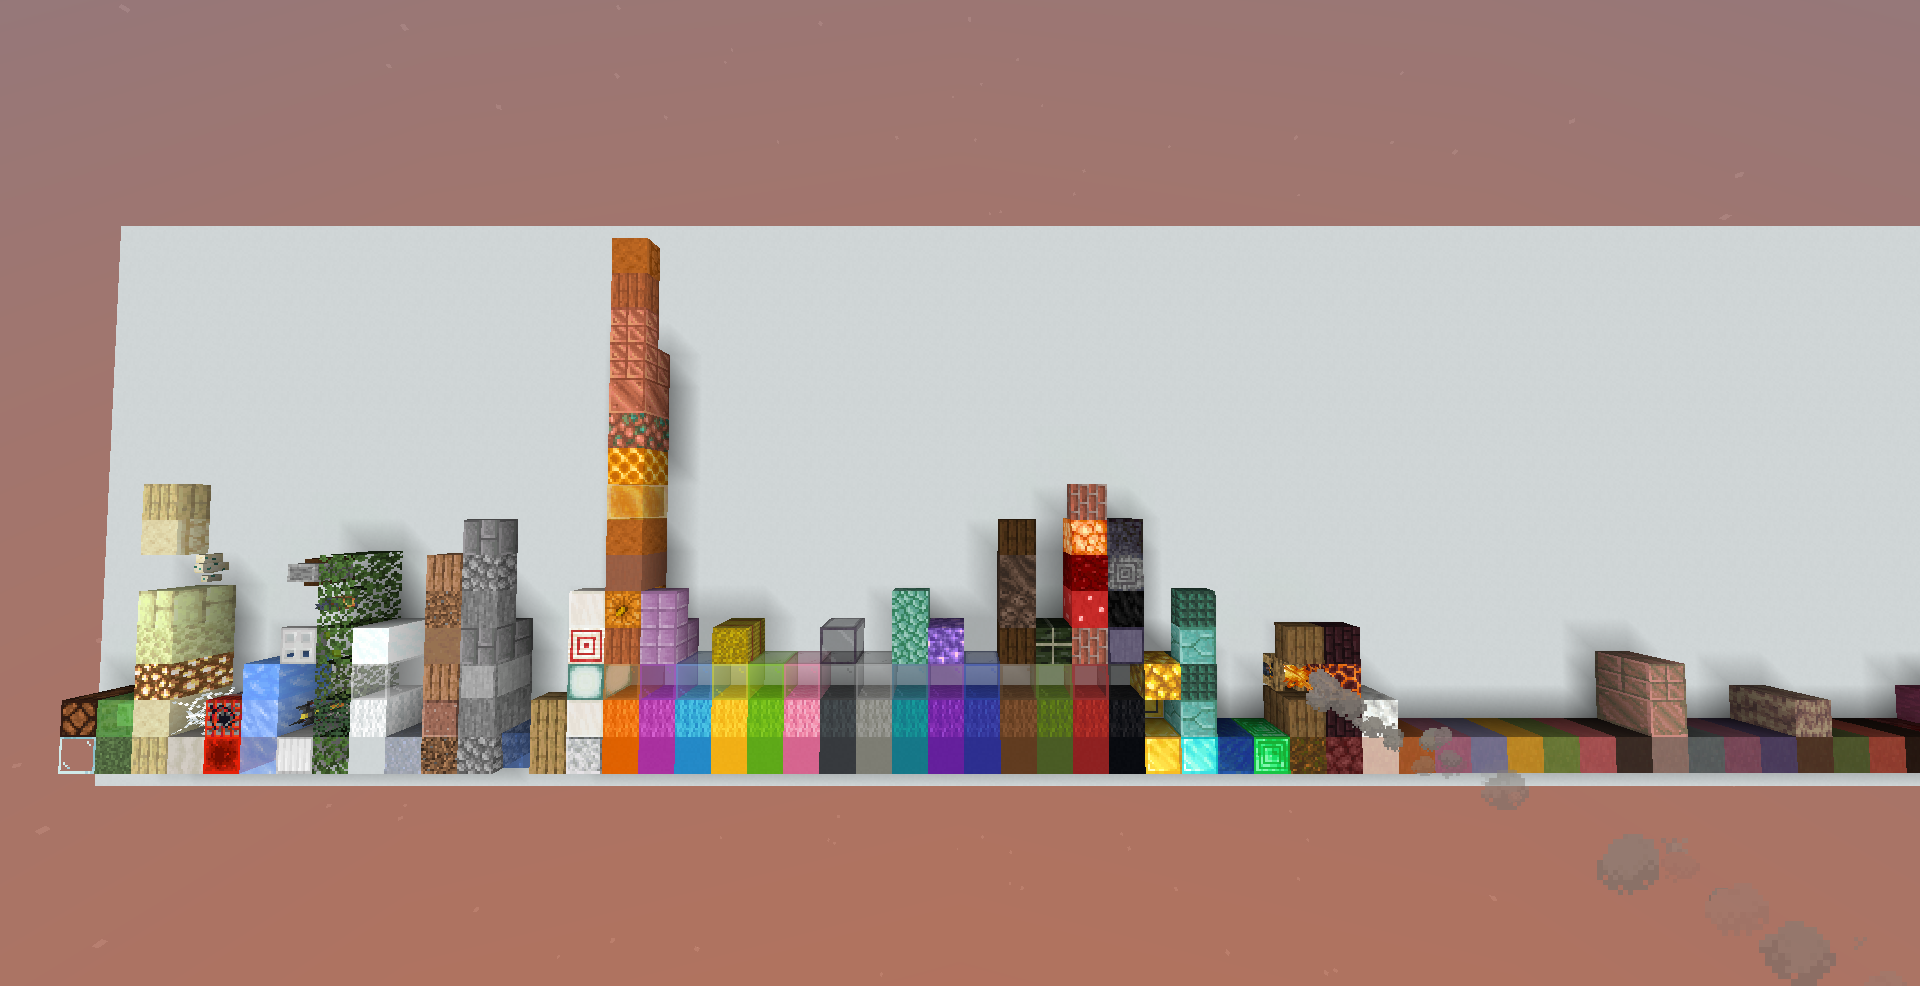
\includegraphics[width=6.5cm]{Img10_TestBlockList_Left.png}
            \end{minipage}
        }
        \subfigure[右半段]{
            \begin{minipage}[t]{7cm}
                \centering
                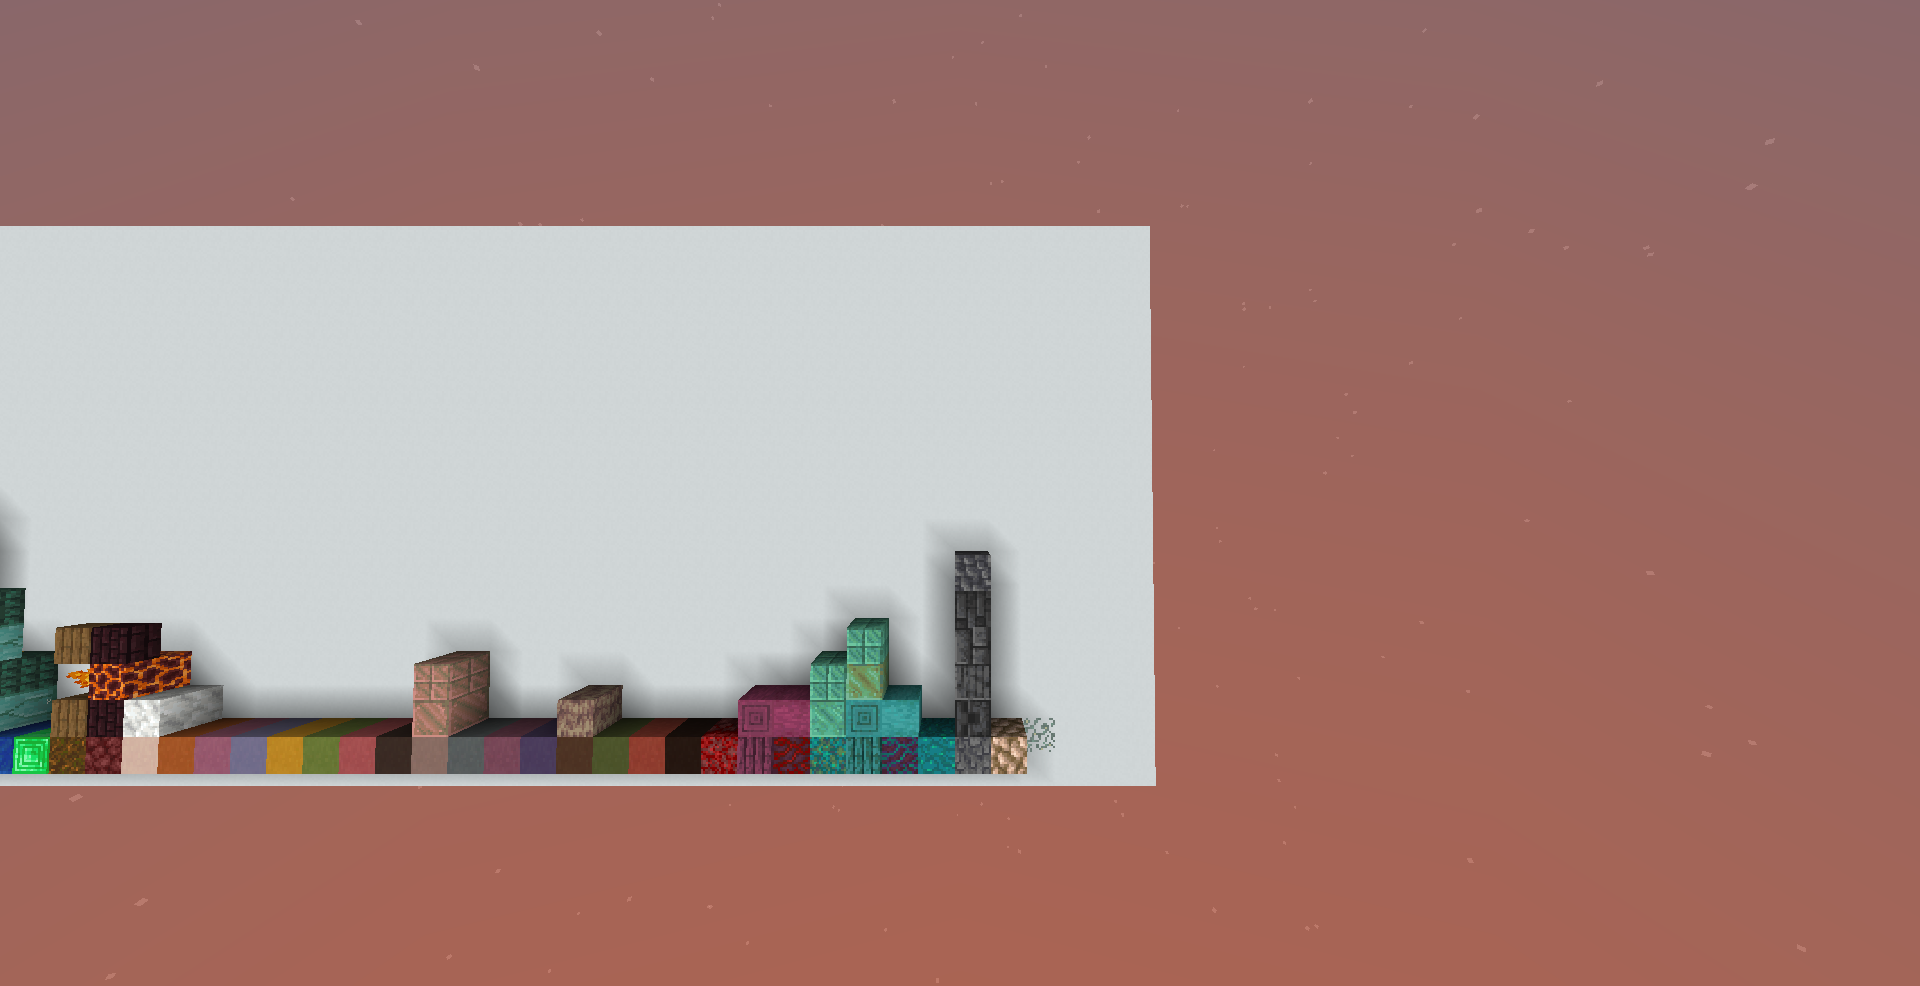
\includegraphics[width=6.5cm]{Img11_TestBlockList_Right.png}
            \end{minipage}
        }
        \caption{测试方块列表}
        \label{testBlockListNBT}
    \end{figure}

%\pagebreak
\section{下个版本}
    不出意外,下个版本v3.7将会加入以下功能:
    \begin{enumerate}
        \item 跟进Minecraft1.18
        \item 批量生成地图画
        \item 手动精修
        \item ……
    \end{enumerate}

\end{document}
